% Intended LaTeX compiler: pdflatex
\documentclass[10pt,a4paper,UTF8]{article}
\usepackage{zclorg}
\usepackage{tikztheorem}
\author{张朝龙}
\date{}
\title{谱定理}
\hypersetup{
 pdfauthor={张朝龙},
 pdftitle={谱定理},
 pdfkeywords={},
 pdfsubject={},
 pdfcreator={Emacs 25.2.1 (Org mode 9.0.9)},
 pdflang={English}}
\begin{document}

\maketitle
\tableofcontents
\titlepic{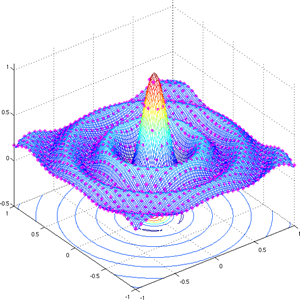
\includegraphics[scale=0.25]{../../img/sinc.PNG}}

\section{简介}
\label{sec:org9a2594a}


回想,对角矩阵是对角线之外的元素都是 0 的方阵:\(V\) 上的算子关于某个基有对角矩阵当且仅当这个基是由该算子的本征向量组成的。

关于\(V\)的某个规范正交基具有对角矩阵的算子是\(V\)上最好的算子,它们恰好是具有如下性质的算子\(T\in \mathcal{L}(V)\):\(V\)有一个由\(T\)的本征向量组成的规范正交基。本文要证明的是谱定理。谱定理表明:具有上述性质的算子当\(\mathbf{F} = \mathbf{C}\)时恰为正规算子,当\(\mathbf{F} = \mathbf{R}\)时,恰为自伴算子。谱定理是研究内积空间上算子的最有用的工具。

由于谱定理的结论依赖于\(\mathbf{F}\),所以我们把谱定理分成两部分,分别叫做复谱定理和实谱定理。同线性代数中的大多数情形一样,处理复向量空间要比处理实向量空间容易,因此我们先分析复谱定理。

\section{复谱定理}
\label{sec:orge57871e}


若\(\mathbf{F} = \mathbf{C}\)且\(T\in \mathcal{L}(V)\)是正规的,则\(T\)关于\(V\)的某个规范正交基具有对角矩阵。

\begin{tikzinstance}
考虑正规算子\(T\in \mathcal{L}(\mathbf{C}^{2})\),它关于标准基的矩阵是:
\begin{equation}
\label{eq:1}
\begin{bmatrix}
  2& -3 \\
  3& 2
\end{bmatrix}
\end{equation}
可以验证,\(\tfrac{1}{\sqrt{2}}(i,1), \tfrac{1}{\sqrt{2}}(-i,1)\)是由\(T\)的本征向量构成的\(\mathcal{C}^{2}\)的规范正交基,\(T\)关于这个基的对角矩阵是:
\begin{equation}
\label{eq:2}
\begin{bmatrix}
  2+3i & 0 \\
  0 & 2-3i
\end{bmatrix}
\end{equation}
\end{tikzinstance}

\begin{tikztheorem}
设\(\mathbf{F}=\mathbf{C}\)且\(T\in \mathcal{L}(V)\),则以下条件等价:
\begin{enumerate}
\item \(T\)是正规的。
\item \(V\)有一个由\(T\)的本征向量构成的规范正交基。
\item \(T\)关于\(V\)的某个规范正交基具有对角矩阵。
\end{enumerate}
\end{tikztheorem}
\begin{proof}
首先假设第 3 条成立,则\(T\)在\(V\)的某个规范正交基下具有对角矩阵。\(T^{*}\)的矩阵是\(T\)的矩阵的共轭转置,所以\(T^{*}\)也具有对角矩阵。任意两个对角矩阵都是交换的,所以\(T\)和\(T^{*}\)是交换的,从而\(T\)是正规的。也就是说第一条成立。

现在假设第一条成立,则\(T\)是正规的。由舒尔定理可知\(V\)有一个规范正交基\(e_{1},\ldots ,e_{n}\)使得\(T\)关于此基有上三角矩阵,于是:
\begin{equation}
\label{eq:3}
\mathcal{M}(T,(e_{1},\ldots ,e_{n})) =
\begin{bmatrix}
  a_{1,1} & \ldots & a_{1,n} \\
          & \ddots & \vdots  \\
    0     &        & a_{n,n}
\end{bmatrix}
\end{equation}
由上面的矩阵可得:
\begin{equation}
\label{eq:4}
\| Te_{1} \| ^{2} = |a_{1,1}|^{2}
\end{equation}
且:
\begin{equation}
\label{eq:5}
\| T^{*} e_{1} \|^{2} = |a_{1,1}|^{2} + |a_{1,2}|^{2} + \ldots + |a_{1,n}|^{2}
\end{equation}
因为\(T\)是正规得,所以\(\|Te_{1}\| = \|T^{*}e_{1}\|\),于是由上面得两个等式可知,式\textasciitilde{}(\ref{eq:3}) 中矩阵的第一行除了第一个元素之外都是 0. 以此类推,\textasciitilde{}(\ref{eq:5})中除了对角线上的元素其他元素都为 0.
\end{proof}
\section{实谱定理}
\label{sec:org3e9e8d3}


\begin{tikztheorem}
设\(T\in \mathcal{L}(V)\)是自伴的,并设\(b,c\in \mathbf{R}\)使得\(b^{2} < 4c\),则:
\begin{equation}
\label{eq:6}
T^{2} + bT +cI
\end{equation}
是可逆的。
\end{tikztheorem}

\begin{proof}
设\(v\)是\(V\)中的非零向量,则:
\begin{eqnarray*}
\langle (T^{2}+bT + cI)v ,v \rangle  &=& \langle T^{2}v,v \rangle +b \langle Tv,v \rangle + c \langle v,v \rangle  \\
&=& \langle Tv, Tv \rangle  + b \langle Tv,v \rangle + c\|v\|^{2} \\
&\geq& \|Tv\|^{2} - |b| \|Tv\| \|v\| + c \|v\|^{2} \\
&=& \bigg( \|Tv\| - \frac{|b|\|v\|}{2} \bigg)^{2} + \bigg( c - \frac{b^{2}}{4} \bigg) \|v\|^{2} \\
&>&0
\end{eqnarray*}
所以\((T^{2} + bT + cI)v \neq 0\),所以\(T^{2} + bT + cI\)是单的,从而是可逆的。
\end{proof}

\begin{tikztheorem}
设\(V\neq \{0\}\)且\(T\in \mathcal{L}(V)\)是自伴算子,则\(T\)有本征值。
\end{tikztheorem}

\begin{proof}
如前所述,可以假设\(V\)是实内积空间。设\(n=\dim V\),取\(v\in V\)使得\(v\neq 0\),则:
\begin{equation}
\label{eq:8}
v,Tv,T^{2}v,\ldots ,T^{n}v
\end{equation}
不可能是线性无关的,因为\(V\)是\(n\)维的,而这里有\(n+1\)个向量。于是,有不全为 0 的实数\(a_{0},\ldots ,a_{n}\)使得:
\begin{equation}
\label{eq:9}
a_{0}v + a_{1}Tv + \ldots + a_{n}T^{n}v
\end{equation}
以这些\(a_{j}\)为系数做一个多项式,并将此多项式分解则:
\begin{eqnarray*}
& &a_{0} + a_{1}x + \ldots + a_{n}x^{n} \\
&=&c(x^{2} + b_{1}x +c_{1}) \ldots (x^{2}+b_{M}x+c_{M})(x-\lambda_{1})\ldots (x-\lambda_{m})
\end{eqnarray*}
其中\(c\)是实数,每个\(b_{j},c_{j},\lambda_{j}\)都是实数,每个\(b_{j}^{2}\)小于\(4c_{j}\),\(m+M \geq 1\),并且上面的等式对所有实数\(x\)都成立。那么我们有:
\begin{eqnarray*}
0&=& a_{0}v + a_{1}Tv + \ldots a_{n}T^{n}v \\
&=& (a_{0}I + a_{1}T + \ldots + a_{n}T^{n})v \\
&=& c(T^{2} + b_{1}T + c_{1}I)\ldots (T^{2} + b_{M}T +c_{M})(T-\lambda_{1}I)\ldots (T-\lambda_{m}I)v
\end{eqnarray*}
每个\(T^{2}+b_{j}T+c_{j}I\)都是可逆的。而\(c\neq 0\),所以上面的等式表明\(m > 0\)且:
\begin{equation}
\label{eq:11}
0 = (T-\lambda_{1}I)(T-\lambda_{2}I)\ldots (T-\lambda_{m}I)v
\end{equation}
所以至少有一个\(\lambda_{j}\)使得\(T-\lambda_{j}I\)不是单的,也就是说\(T\)有本征值。
\end{proof}
\end{document}
